\section{Binary Classification and Linear Regression}
A binary classification problem has only two possible outcomes: yes, no. The algorithm for solving binary classification is logistic regression.\\
Optimize the model using the probabilities and not the response. In other words: We want a cost function over probability of classmembership y.

\subsection{Binary Classification}
Why not with linear regression? LR optimizes the wrong quantity.\\
\textbf{Problems:} Using LR, we model the response (y) and post process the response (e.g. by thresholding) to compute the probability. $\rightarrow$ The cost function minimizes the MSE difference in the values of $\hat{y}$ and y and has nothing to do with the clasification probabilities.

\subsection{Logistic Regression}
 The sigmoid function maps all input to a probability. This is where our features (data x) enters the calculation. The weights are unknown and need to be learned. 
$y=w_{1} x_{1}+w_{2} x_{2}...$

\begin{minipage}{0,6\linewidth}
	Can work with continous data and discrete data.
	\[ sigmoid(y) = \frac{1}{1+ e^{-y}} \] 
	The weights is a model parameter. \\
	$Pr(y=1|(feature vector); (Weights))$\\
	\[ Pr(y=1|x) = Pr(y=1|x) = p(x) = \frac{1}{1+e^{-(W^{T} x_{i})}} \]
	W is a vector can be found with Maximum Likelihood. 
\end{minipage}
\begin{minipage}{0,4\linewidth}
	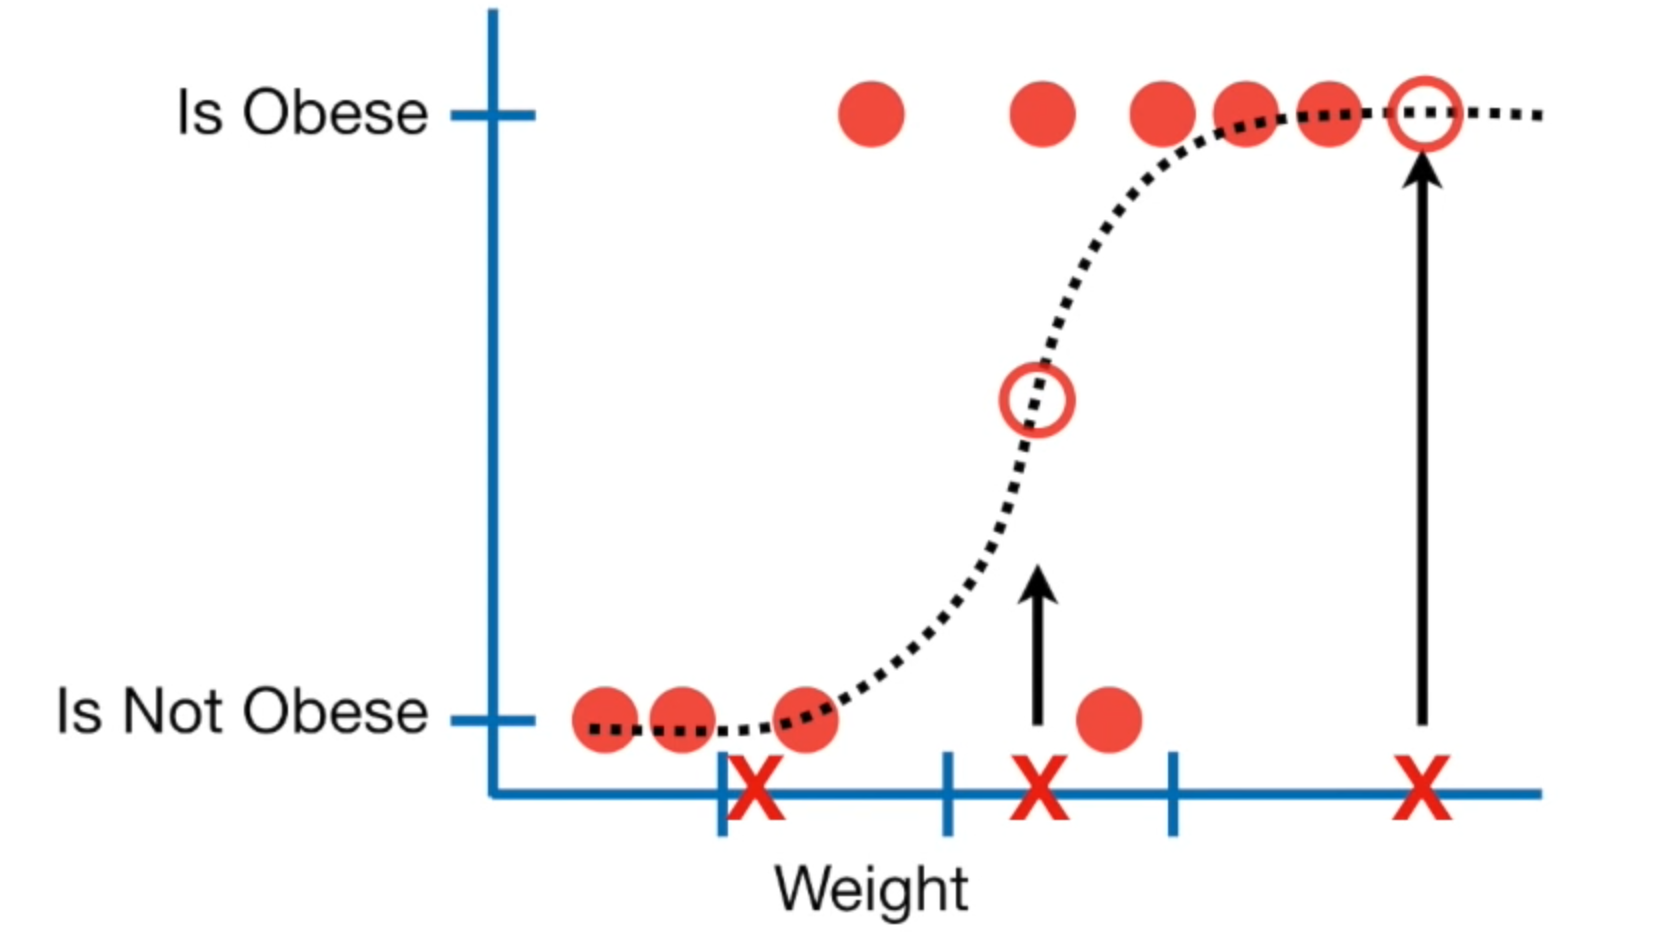
\includegraphics[width=\linewidth]{logisticregression}
\end{minipage}

\subsection{Maximum Likelihood}
Given all the data points (X, Y) we want to maximise the probability that all the predictions are correct. The objective off the training is to set the coefficients W so that: p is close to 1 when y=1 and p is close to 0 when y=0. To find the perfect W we can use Gradient Descent.
\[ Maximum Cost_{2}(W) = \sum_{y=1}^{N} \log(p(x_{i}) + \sum_{y=0}^{N} \log(1-p(x_{i})) \]



